\documentclass[letterpaper]{article}
\usepackage{natbib,alifexi}
\usepackage[utf8x]{inputenc}

\usepackage{xcolor}

\title{Plan-Based Reward Shaping for Multi-Agent Reinforcement Learning}
\author{Jérôme Bastogne$^{1}$, Maxime Desclefs$^{1}$ \and Simon Picard$^{1}$ \\
\mbox{}\\
$^1$Université Libre de Bruxelles, Boulevard du Triomphe - CP 212, 1050 Brussels, Belgium \\
jbastogn@ulb.ac.be, mdesclef@ulb.ac.be, spicard@ulb.ac.be}


\begin{document}
\maketitle

\begin{abstract}
Reward shaping is known to significantly improve an agent’s performance in multi-agent reinforcement
learning (MARL). This paper shows the benefits of using plan-based reward shaping in which a STRIPS planning knowledge is used. The results of agents using plan-based reward shaping will then be compared to a simple Reinforcement Learning (RL) agent with no domain knowledge and they will show how they outperform previous results.
\end{abstract}

\section{Introduction}

Reinforcement learning agents don't get future feedback about how good was their decision taken in a precise state. This leads to a temporal problem as the agents will not know immediately which part of their decisions where the good ones \citep{rs}. RL, while being simple, presents some issues. The time taken by the agents to learn the right policy grows exponentially while adding new variables to the environment. When the state space is too vast, memory becomes an issue as well as the matrix for each state-action pair becomes too big and too many states need to be updated too frequently slowing down drastically the process. 

A way of improving the converging speed is to provide prior knowledge to the agents through a method called reward shaping. Reward shaping is the addition of domain knowledge to reinforcement learning in a way that will minimize non-optimal behaviours and will fastly converge to the optimal one. In this article we will see how to effectively incorporate reward shaping in MARL using individual and joint plan based plans and we will combine them with a flag based heuristic\citep{paper4}.

We will show that providing prior knowledge, while not always being possible due to heuristic problems, significantly increases agent's performances and speed of convergence.

\section{Study Case}

We choose two agents who starts on the S1 and S2 squares respectively. Their objective is to reach the goal while trying to collect a maximum of flags while doing so. At each time step, they will move one square up, down, left or right unless they collide with a wall or the other agent. Each of our agents has to reach the goal to end an episode. When an agent reaches the goal, his episode is over and he will wait the other agent to finish his run. For the initial case, when they both reach the goal, they receive a reward equal to $100*NumFlagsCollected$. 

\begin{figure}[h!]
\centering
  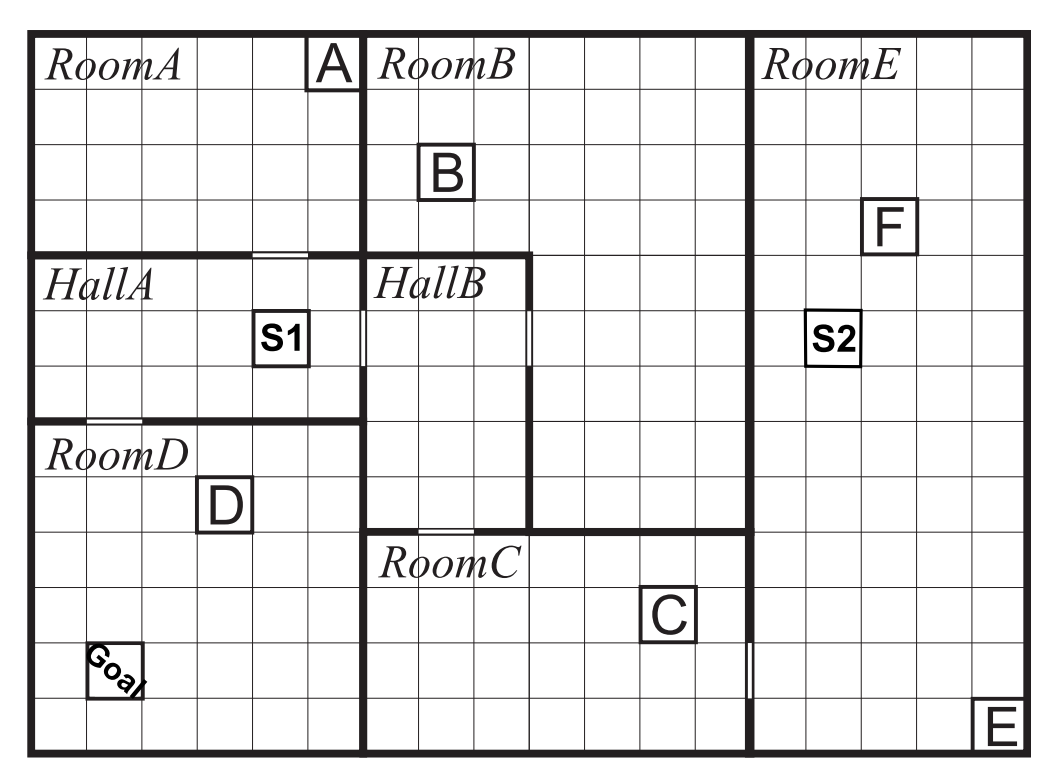
\includegraphics[width=0.75\linewidth]{img/stydyCase.png}
  \caption{Multi-Agent, Flag-Collecting Problem Domain.}
  \label{fig:studycase1}
\end{figure}



\section{Materials and Methods}
\subsection{Reinforcement Learning}
Reinforcement learning is a method of rewarding an agent for taking a good decision in a particular state. The better state the decision leads to, the better that decision will be rewarded. Therefore RL can be considered as a Markov Decision Process. Each agent remembers what rewards he got for each action in each state. 

The possible actions here are going up, down, left and right. A state here, is a position (x, y) in the world space combined the current step in the plan. To each of these Q(s,a) state-action pairs is associated a Q-value translating the goodness of choosing that action while being in that state. The reinforcement algorithm is iterative and dynamic, therefore agents have to run multiple episodes where they have to reach the goal and where they are rewarded depending on the number of flags they got together. At each step, we need to update Q(s,a)  for future learning. A way of achieving this is by applying a temporal-difference update to Q(s,a) so that Q(s,a) will increase only if it leads to a better state than the actual one. This ensures that agents are willing of doing better while reaching the goal. There is an algorithm called SARSA that does this by updating Q-values as follows : \\

$Q(s, a) \leftarrow  Q(s, a) +  \alpha [r + \gamma Q(s', a') - Q(s,a)]$\\\\
where $\alpha$ is the rate of learning and $\gamma$ is the discount factor. r is the reward returned by the environment. In our case, rewards will only be given when agents reach the final goal. 

At the beginning, agents know nothing about their environment, therefore they will randomly travel through the world space. After few iterations some of their actions will have positive rewarded scores but might not be the most optimals. Therefore, a good balance between exploration and exploitation of the best rewarded actions must be found. The most common method is by using the $\epsilon$-greedy algorithm. It ensures that at each step, the best value action will be chosen with a probability 1- $\epsilon$ and otherways, the agent will explore a new action.


A well-known method to fasten this process is eligibility traces. When a reward is received, the lasts state-actions pairs that the agent has been walking through are also updated according to their temporal difference with the last state-action pair. Each Q-value in the current's agent's path is updated as follows : \\

$Q(s, a) \leftarrow  Q(s, a) +  \alpha *  \sigma (\gamma * \lambda)^t$\\\\
where $\lambda$ has to be lower or equal to 1 \citep{etrace}. Where $ \sigma = r + \gamma Q(s', a') - Q(s,a)$ We choosed  $\lambda = 0.4$ for our experiment.

\subsection{Reward Shaping}

Reward shaping is a method in reinforcement learning that attributes additionnal rewards to the agents that should guide them to find their optimality and in a much faster way.
The addition of reward shaping to reinforcement learning changes the SARSA algorithm formula as follows: \\

$Q(s, a) \leftarrow  Q(s, a) +  \alpha [r + F(s, s') + \gamma Q(s', a') - Q(s,a)]$\\\\
where $ F(s, s')$  is a difference of potentials defined as follows : \\

$F(s, s') =\gamma \phi (s') - \phi (s)$\\\\
where $\phi$ is some function over states. The difference of potentials is usefull for avoiding cycles  \citep{rs2}.

\subsection{Plan-Based Reward Shaping}

For plan-based reward shaping, agents are given STRIPS plans that transposes into a list of states as shown on  Figure \ref{fig:strips}.

\begin{figure}[h!]
\centering
  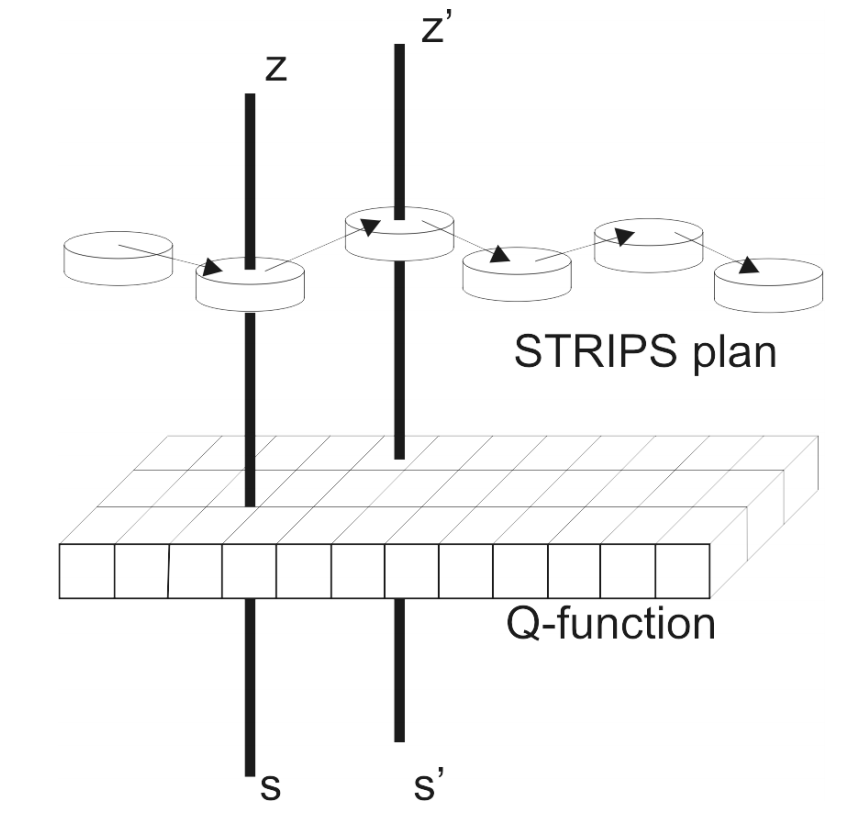
\includegraphics[width=0.75\linewidth]{img/strips.png}
  \caption{Plan-base reward shaping.}
  \label{fig:strips}
\end{figure}


It consists in a set of subgoals that the agent should be focusing on in the specified order to increase the total ending reward. In our experiment, subgoals are : going from a room to another, and collecting a flag in the current room when specified. Examples of individual and joint plans we will be using are given on figures \ref{fig:plan1} and \ref{fig:plan2}.

\begin{figure}[h!]
\centering
  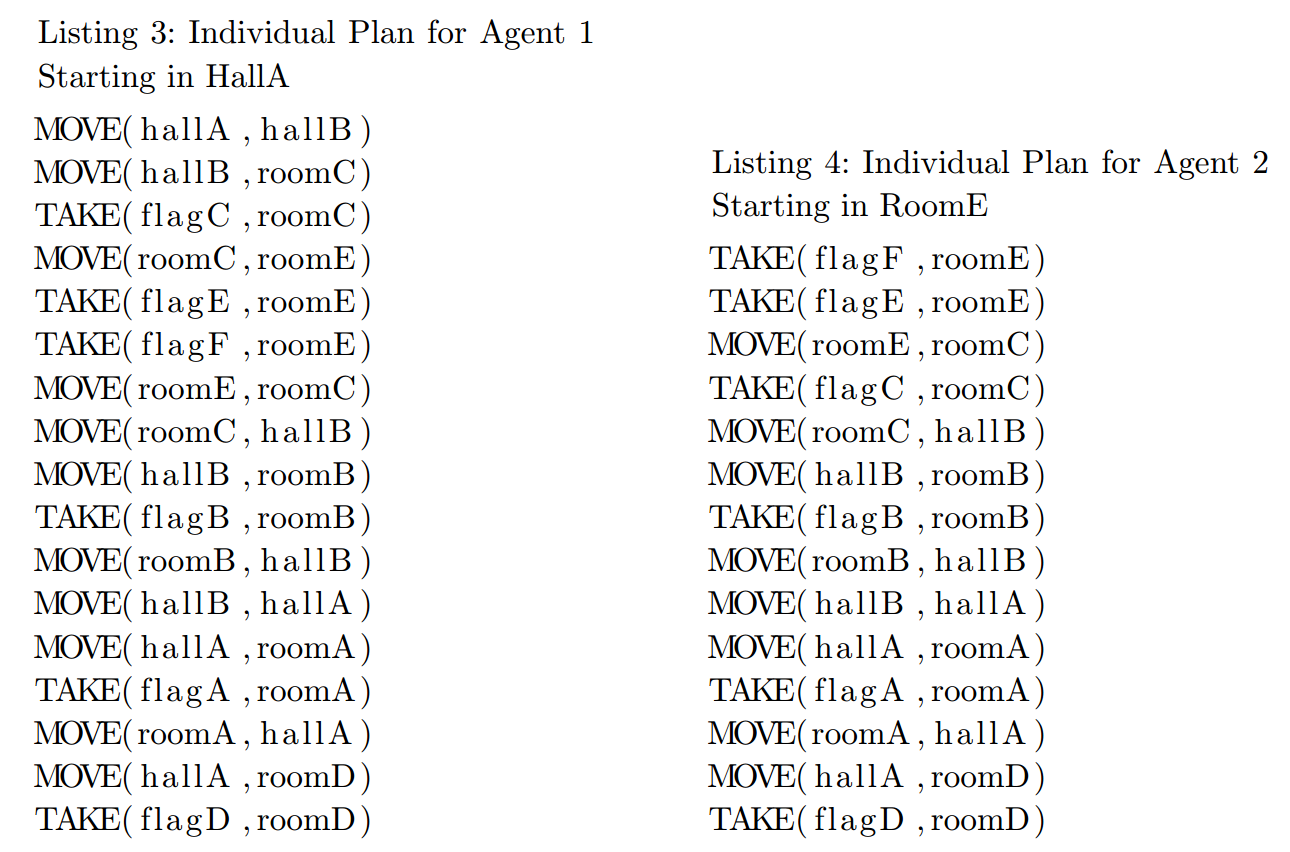
\includegraphics[width=0.85\linewidth]{img/individualPlan.png}
  \caption{Individual plan.}
  \label{fig:plan1}
\end{figure}

\begin{figure}[h!]
\centering
  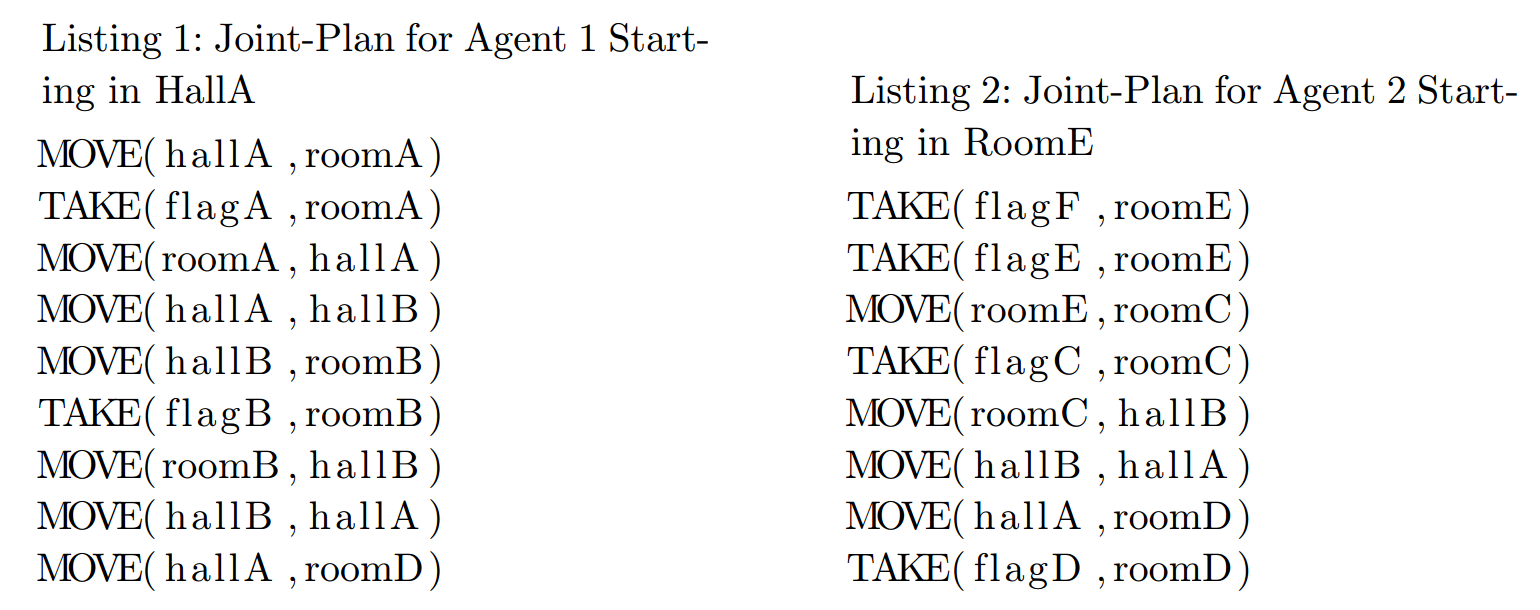
\includegraphics[width=0.85\linewidth]{img/joinPlan.png}
  \caption{Joint plan.}
  \label{fig:plan2}
\end{figure}

Each of these plans are translated into a sequence of states that the agent should follow as a state-based plan (Figure \ref{fig:plan3}). 

\begin{figure}[h!]
\centering
  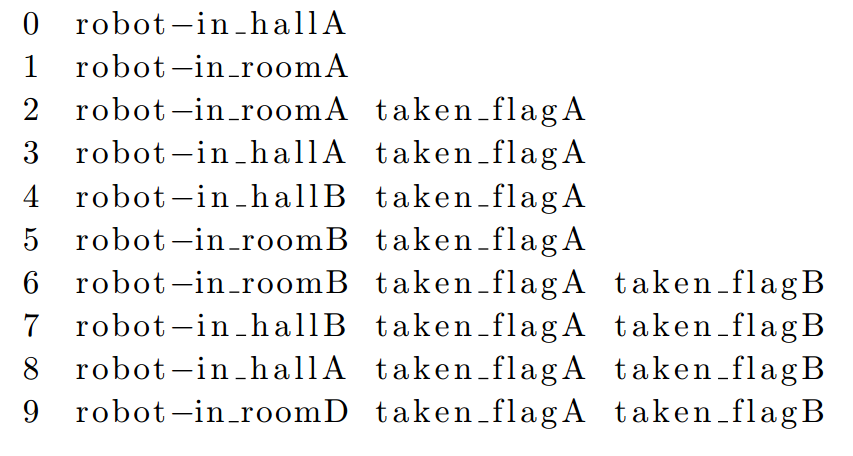
\includegraphics[width=0.85\linewidth]{img/listingFormattedJoinAgent1.png}
  \caption{State-Based Joint-Plan.}
  \label{fig:plan3}
\end{figure}

The agent's potential $\phi$ can be chosen as :\\

$\phi (s) = \omega * CurrentStepInPlan$

$\omega = MaxReward/NumStepsInPlan$\\\\
where $\omega$ is a scaling factor and $CurrentStepInPlan$ is the corresponding plan's step of the agent's state. We will compare the differences between individual and joint plan based reward shaping and we will see the benefits and constraints of each.

When running the combination of flag-based method with individual-plan-based and joint-plan-based shaping, the agent's potential becomes :\\

$\phi (s) = \omega * (CurrentStepInPlan + NumFlagsCollected)$

$\omega = MaxReward/(NumStepsInPlan + NumFlagsInWorld)$\\\\
where $NumStepsInPlan$ is the number of step in its state-based plan, $NumFlagsInWorld$ is the total number of flags in the world and $NumFlagsCollected$ is the number of flags the agent has collected itself.

\section{Results and Discussion}
\subsection{Initial results}

After running thirty times all experiments, the mean discounted reward per episode were plotted on the following graphs. The discounted reward is the goal reward multiplied by the discounted factor exponent the step number needed to reach the goal  \citep{SCpbrs}. This value offers a way to classify the shaping, taking into account the number of flags collected and the time the agents takes to get them.\\
 Our initial case results are shown on Figure \ref{fig:results1}. \\

\begin{figure}[h!]
  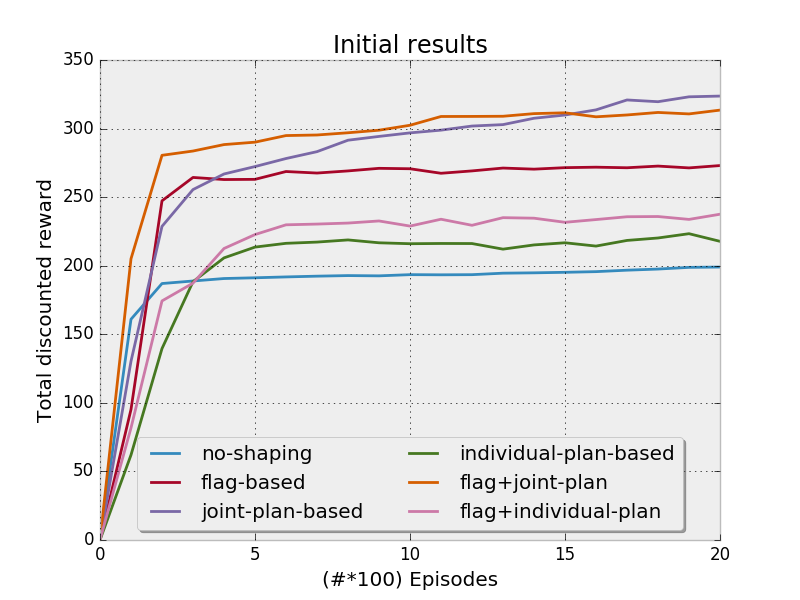
\includegraphics[width=\linewidth]{img/initial.png}
  \caption{Initial results.}
  \label{fig:results1}
\end{figure}

First, it is shown on the results that the learning with no shaping gives the worst outcome. This result was the expected one since knowledge, even poor, improves the behaviour of the agents.\\
Next, as one can see, the joint-plan-based gives the best result. With the joint-plan, the agents cooperates to collect the six flags, i.e the optimal way.\\
About the individual-plan-based shaping, the discounted reward is rather low, just above the no shaping one. This results comes from two main behaviours of the agents with this plan. When analysing the individual plans, one will quickly notice that the agents will jeopardize each other early. Indeed, each agent will try to collect the flag that the other agent needs to collect, they will find themselves in a deadlock situation. The other possible outcome is when agent number two takes all the flags and the other one none as it can be seen on figure \ref{fig:behave}.\\
The flag-based reward shaping get the agents to learn a behaviour where they collect the flags that are on their path leading to a result where the agent goes quickly to the goal but with approximately two third of the flags.\\
When adding the flag-based heuristic to the plan-based one, for the joint-plan it converges quicker but then doesn't give significant differences since the results without it are already optimal. For the individual-plan-based reward shaping, it is clear that it improves the reward a bit because it adds some knowledge to the agents.\\

\begin{figure}[h!]
  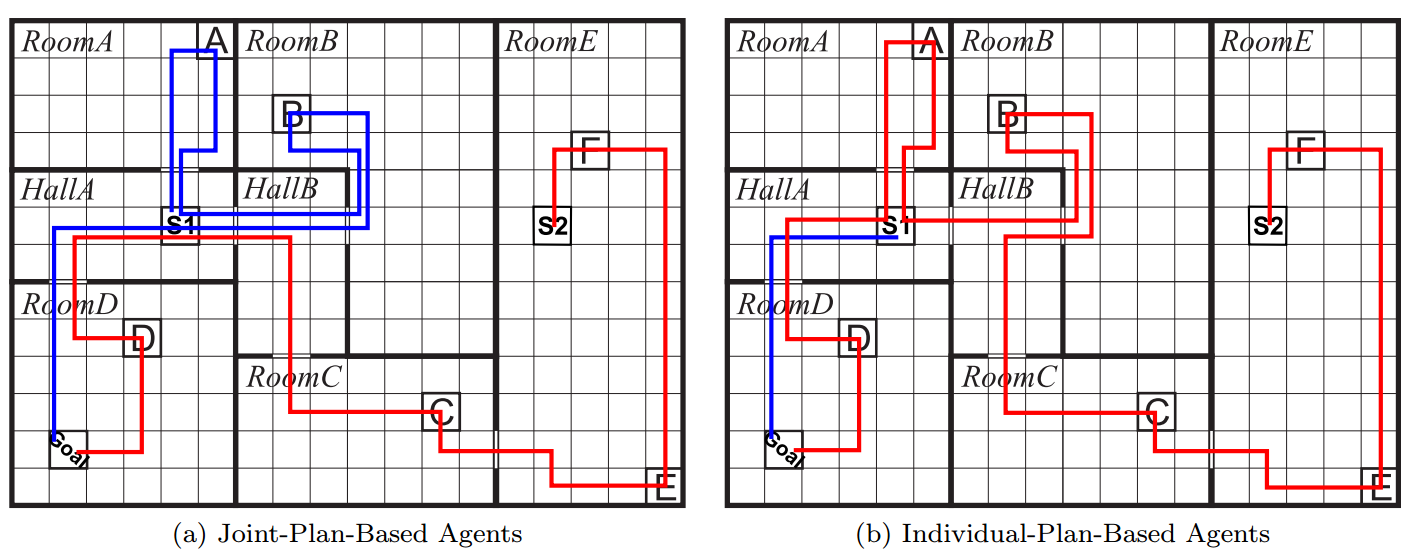
\includegraphics[width=\linewidth]{img/behavious.png}
  \caption{Behaviours of :}
  \label{fig:behave}
\end{figure}

Once obtaining those result, our aim was to reduce the gap between the results of the plan based reward shaping with joint plan and individual plan.\\
In order to do so, we explored two methods. The first one is about improving the knowledge of the agents and the second one concern their cooperation.

\subsection{Improved knowledge}

In this section, the idea is to improve the knowledge of the agents by altering their plan.\\
One should bear in mind that the aim is to tend to the results given by the join plan based rewards shaping since it gives the best output.\\
We saw that one major issue of the individual plan based heuristic, is the conflict knowledge. We therefore tried to reduce it.\\
The first way was to delay the conflict in the plan to the fifth collected flag whereas it is the fourth flag in the original plan.\\
The other new plan, are also individual but they make the agents collect only five or four flags, thus there is only four or two common flags left.\\
In the following graph, one will find the results of those new plan, compared with the no shaping one and the joint plan based one. The delayed conflict is represented by plan-based-6 and the two other shaping heuristics represent the one where the individual plans do not take all the flags.

\begin{figure}[h!]
  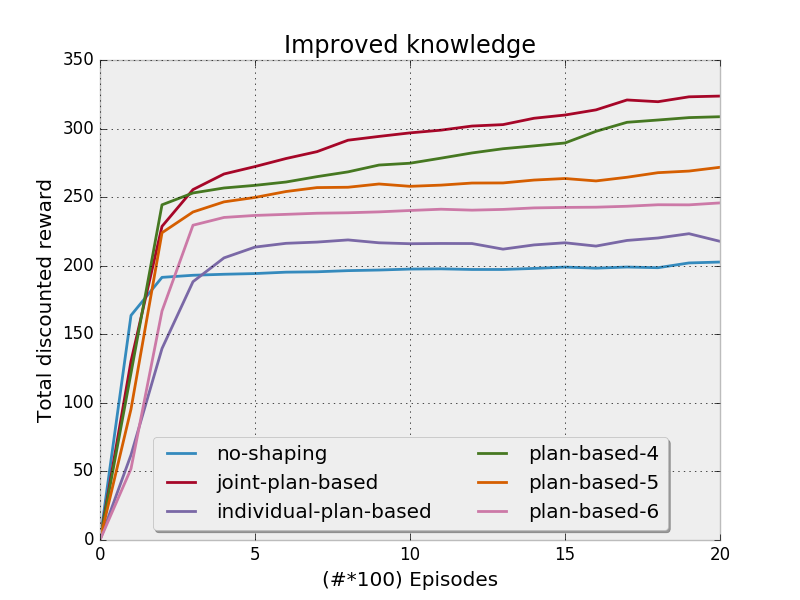
\includegraphics[width=\linewidth]{img/knowledge.png}
  \caption{Improved knowledge.}
  \label{fig:results2}
\end{figure}

\subsection{Improved cooperation}

\begin{figure}[h!]
  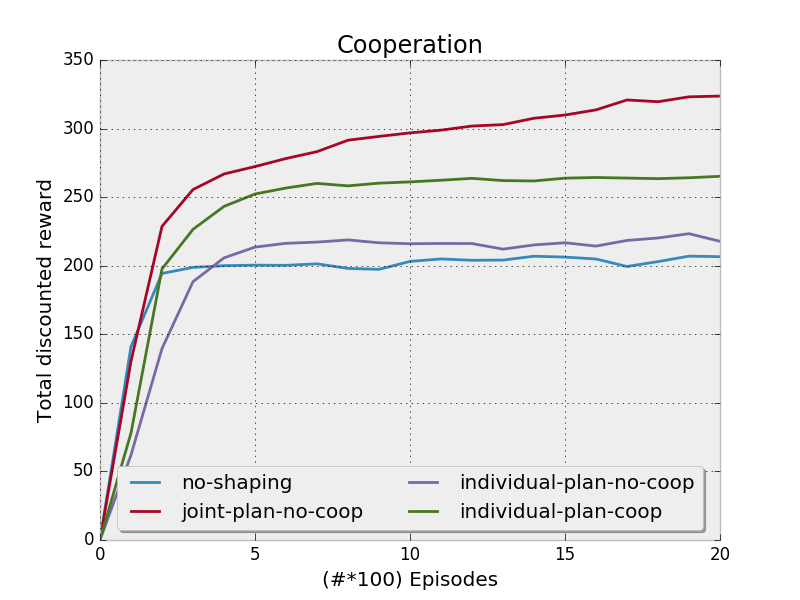
\includegraphics[width=\linewidth]{img/coop.png}
  \caption{Improved cooperation.}
  \label{fig:results3}
\end{figure}

\section{Conclusion}




\footnotesize
\bibliographystyle{apalike}
\bibliography{example}


\end{document}
